\begin{figure}
    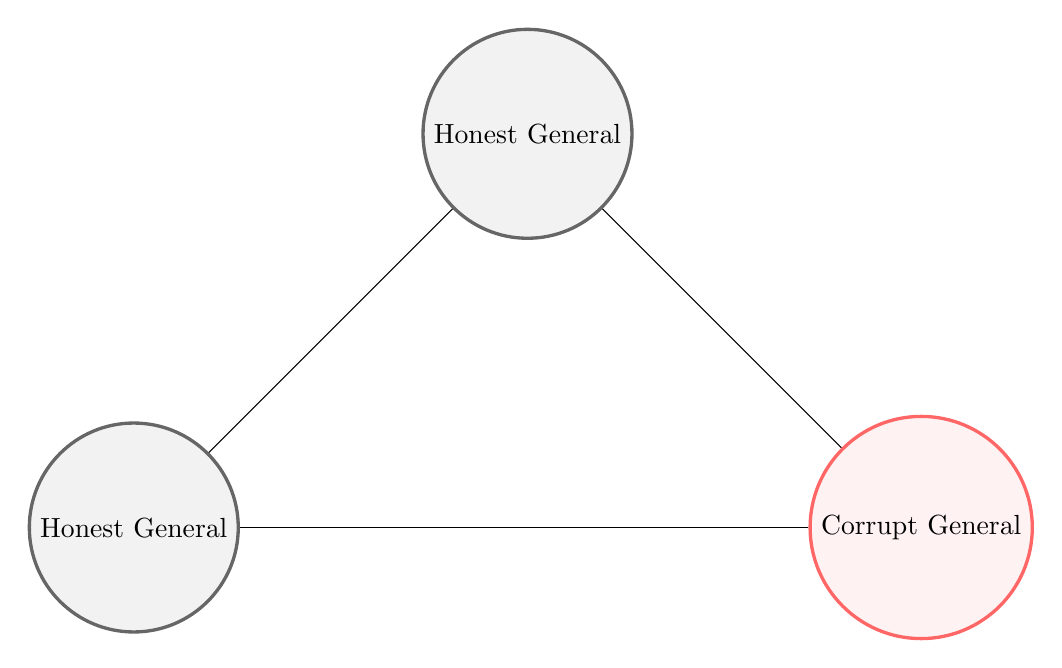
\begin{tikzpicture}[
        roundnode/.style={circle, draw=black!60, fill=black!5, very thick},
        rednode/.style={circle, draw=red!60, fill=red!5, very thick},
        ]

        % Nodes
        \node[roundnode] (a) at (0,0) {Honest General};
        \node[rednode]   (b) at (10,0) {Corrupt General};
        \node[roundnode] (c) at (5,5) {Honest General};
       
        \draw[] (a) -- (b);
        \draw[] (b) -- (c);
        \draw[] (c) -- (a);

    \end{tikzpicture}

    \label{fig:byzantine}
    \caption{
        An illustration of the Byzantine Generals Problem. The Theorem states that consensus cannot be reached if 1/3 or more are malicious.
    }
\end{figure}
